\section{RxJS: Reactive Extensions For JavaScript}

Rx ist eine Library, die für zahlreiche Programmiersprachen zur Verfügung gestellt wird. Diese finden sowohl in der Frontend als auch in der Backend-Implementierung Anwendung. In dieser Arbeit wird der Fokus auf RxJS geworfen. Diese Library ist eine Erweiterung speziell für Javascript/Typescript. RxJS erlaubt es mit Hilfe von Observable-Sequenzen Event-basierte Programme zu erstellen. Dabei wird dieser Ansatz auch als \textbf{reactive Programming} definiert. Neben der Kernfunktionalität von Observables werden auch Subjects und Schedulers geboten. Sollte man von reactive Programming noch nichts gehört haben, dann wird die größte Herausforderung sein \glqq{}reactive\grqq{} zu denken.

\subsection{Reactive Programming}
Im Kern ist reactive Programming ein Programmierparadigma. Im \textbf{reaktiven Manifest}, zu finden unter

\begin{center}
\url{https://www.reactivemanifesto.org/de},
\end{center}

\noindent
wird bereits beschrieben, dass Reactive Programming als Programmierung mit asynchronen, unveränderlichen Streams von Events bezeichnet wird. Laut der offiziellen Dokumentation richtet sich ReactiveX nach dem Beobachter-Muster (engl. Observer-Pattern). Das Observer-Pattern ist ein Entwurfsmuster, in der Änderungen eines Objektes (Subjects genannt) an einer Liste abhängiger Strukturen weitergereicht wird. Diese abhängige Strukturen (Observers) werden bei jeder Zustandsveränderung informiert. Eine Veränderung eines Objekts kann hierbei gleichgesetzt werden mit einem neuen Wert innerhalb eines Datenflusses. Als Beispiel für eine reaktive Anwendung kann Excel genommen werden. Ändert man einen Wert in einer Zelle, ändert sich auch der Wert in der Summenzelle. Die Zelle, deren Wert geändert wurde, löst ein Event aus, den die Summen-Zelle empfängt. Daraufhin findet eine Neuberechnung statt\cite{reactive-programming-beispiel}. Datenflüsse können aus verschiedensten Operationen entstehen wie z.B. Klick-Events, Variablen, Cache etc. Als Observer kann man sich in diesem Datenfluss einhängen und entsprechend reagieren\cite{rx-intro}. Rx bietet eine enorme Menge an Funktionen diese Datenflüsse zu bearbeiten/manipulieren. Diese Operatoren komplett abzudecken wird in dieser Arbeit unmöglich sein, jedoch wird nach dem behandeln dieses Kapitels ein gewisses Grundverständnis für neue Operatoren entstehen und wie diese in Folge anzuwenden sind. Die grundlegenden Konzepte, um asynchrone Events in RxJS zu steuern, sind:

\begin{description}
    \item Observable: Repräsentiert die Idee einer abrufbaren Sammlung, in der zukünftige Werte oder Events gelagert sind.
    \item Subscription: Repräsentiert das Aufrufen eines Observable.
    \item Observer: Ein Objekt, dass eine Sammlung von Callbacks enthält, um die aus dem Observable gelieferten Werte, zu verarbeiten.
    \item Operators: Funktionen, die das Verhalten von Observable-Streams beeinflussen.
    \item Subjects: Eine spezielle Form von Observable, die sowohl als Observer als auch als Observable fungiert. Im Gegensatz zu Observables, sind Subjects standardmäßig multicasting fähig.
    \item Schedulers: Steuerungsmechanismen die bestimmen, wann eine Subscription startet und wann Werte aus dem Stream an die Observer übermittelt werden.
\end{description}

\noindent
In dieser Arbeit wird der Fokus hauptsächlich auf Observables und dessen Nutzung mit Operatoren gelegt. Die Einführung von Subjects und Schedulers wird nur oberflächlich thematisiert. Am Ende dieser Sektion wird noch ein zusätzliches Praxisbeispiel dargestellt. Es wird eine Wikipedia Such-App entwickelt, die nach jedem Tasten-Event einen API Aufruf initiiert und das Ergebnis der Suche in Form von Artikel-Snippets präsentiert. Die reine Logik hinter dieser Anwendung wird mit zehn Zeilen Code implementiert.

\subsection{Observables}

Observables sind eine träge Sammlung von multiplen Werten. Sie füllen den fehlenden Platz in der unten stehenden Tabelle:

\begin{center}
    \begin{tabular}{| l | l | l |}
    \hline
    & \textbf{Einzelne-} & \textbf{Multiple Werte} \\ \hline
    \textbf{Pull/synchron} & Funktionen & Iterables (Arrays, Strings, ...) \\ \hline
    \textbf{Push/asynchron} & Promises & Observables  \\ \hline
    \end{tabular}
\end{center}

\noindent
Das Push- und Pull-Prinzip beschreibt dabei wie ein Datenproduzent mit dem Datenverarbeiter kommuniziert. In \textbf{Pull-Systemen} bestimmt der Verarbeiter, wann die Daten vom Ersteller angenommen werden. Der Ersteller selbst weiß nicht, wann die Daten angefragt werden. Jede Javascript Funktion unterliegt einem Pull-System. Die Funktion ist ein Verarbeiter von Daten und diese kann im Code jederzeit abgerufen werden. Das \textbf{Push-Prinzip} wird im nächsten Beispiel deutlich. 

\begin{figure}[H]
\begin{lstlisting}[basicstyle=\small]
module.exports = {
    mode: 'development',
    entry: './src/modules/rxjs/introduction.ts',
    ...
}
\end{lstlisting}
\caption{Im Folgenden muss ../rxjs/introduction.ts als Eingangsdatei definiert werden.}
\end{figure}

\begin{figure}[H]
\begin{lstlisting}[basicstyle=\small]
const alias: Observable<number> = RxJS.Observable.create((observer) => {
    observer.next(1);
    observer.next(2);
    observer.next(3);
    setTimeout(() => {
        observer.next(4);
        observer.complete();
    }, 1000);
});

console.log('Before subscribe');
alias.subscribe(next: x => console.log('Value: ' + x));
console.log('After subscribe');
\end{lstlisting}
\caption{Erstellung eines Observables.}
\label{creation-of-observable-first-example}
\end{figure}

\noindent
Das Observable-Objekt repräsentiert eine Kollektion die Werte zu seinen Beobachtern liefert. In diesem Beispiel wird ein Observable erstellt, dass sofort (synchron) die Werte 1, 2 und 3 produziert, sobald die Subscription gestartet wird. Der vierte Wert wird asynchron übermittelt und das Observable daraufhin geschlossen. Die Konsole gibt die Werte in folgender Reihenfolge aus:

\begin{figure}[H]
\begin{lstlisting}
Before subscribe
Value:  1
Value:  2
Value:  3
After subscribe
Value:  4
Done!
\end{lstlisting}
\caption{Observable können sich sich sowohl synchron als auch asynchron verhalten.}
\end{figure}

\noindent
In Push-Systemen steuert der Datenproduzent, wann die Daten an die Datenverarbeiter übermittelt werden. Der Verarbeiter weiß hingegen nicht, wann die Daten ankommen. Promises sind ein typisches Beispiel für Push-Systeme. Ein Promise (Produzent) übermittelt einen eingetroffenen Wert an angeschlossene Callbacks (Verarbeiter). Ungleich wie mit Funktionen bestimmen Promises, wann die Werte an die Callbacks weitergereicht wird. Observables zählen zu einem neuen Push-System in Javascript. Im Gegensatz zu Promises emittieren Observables multiple Werte in Form von Streams. Zur Unterscheidung:

\begin{description}
\item Eine Funktion ist eine träge ausführende Operation, die beim Abruf ein Wert synchron zurückgibt.
\item Ein Promise ist eine Operation die einen eventuell eintreffenden oder nicht-eintreffenden Wert zurückgibt.
\item Ein Observable ist eine träge ausführende Operation, dass synchron oder asynchron keine oder potenziell unendlich viele Werte ab dem Zeitpunkt des Aufrufs zurückgibt.
\end{description}

\noindent
Hierbei stellt sich die Frage, was bedeutet träge? Träge Funktionen, im englischen auch als \textit{lazy Functions} bezeichnet, sind Funktionen die erst bei ihrem Aufruf Werte produzieren\cite{lazy-functions}.

\begin{figure}[H]
\begin{lstlisting}[basicstyle=\small]
function foo() {
    console.log('Hello');
    return 42;
}

const x = foo();
console.log(x);

const bar = RxJS.Observable.create((observer) => {
    console.log('Hello');
    observer.next(42);
});

bar.subscribe((x) => console.log(x));
\end{lstlisting}
\caption{Mit der subscribe() Methode schließen sich Observer einem Observable Stream an.}
\end{figure}

\begin{figure}[H]
\begin{lstlisting}
Hello
42
Hello
42
\end{lstlisting}
\caption{Der Output bleibt immer derselbe.}
\end{figure}

\noindent
Das liegt daran, da sowohl Funktionen als auch Observables träge sind. Die Operationen innerhalb beider Typen findet erst beim Aufruf statt. Mit anderen Worten: Das starten einer Subscription ist analog zum Aufruf einer Funktion. Entgegen der Annahme, dass Observables ausschließlich asynchron operieren, können diese ebenfalls synchron Werte ausgeben (siehe Abb. \ref{creation-of-observable-first-example}). Der Hauptpunkt in dem sich Observables von Funktionen unterscheiden ist, dass Observables mehrere Werte (mit der Zeit) emittieren können. Innerhalb einer Funktion ist es nicht Möglich zwei return Ausdrücke zu schreiben, die zusammen aufgerufen werden.

\subsubsection{Anatomie eines Observable}
Observables werden entweder mit einer der statischen Methoden, mit einer Observable Instanz oder mit der Hilfe eines Observable-Operators \textbf{erstellt}. Der Datenfluss wird an die Observer mit der subscribe() Methode \textbf{überreicht}. Letzteres kann die Exekution der Datenübertragung \textbf{abgesetzt} werden.

\begin{figure}[H]
\begin{lstlisting}[basicstyle=\small]
const randomNumber = new Observable<number>(observer => {
    observer.next(Math.random());
    observer.complete()
});
\end{lstlisting}
\caption{Instantiierung eines Observables, als Parameter wird ein Callback angenommen.}
\end{figure}

\noindent
Die statische Methode Observable.create() ist ein alias ist zum Konstruktoraufruf. Da Observables kein, ein oder unendlich viele Werte ausstoßen können, gibt es Einschränkungen wie Werte an die Observer verteilt werden. Diese Einschränkungen richten sich nach dem sog. \textit{Observable Contract}. Zum Beispiel ist es nicht möglich nachdem Auftreten eines Fehlers oder Fertigstellung eines Observables noch weiter Werte auszugeben:

\begin{figure}[H]
\begin{lstlisting}[basicstyle=\small]
const observable = new Observable<number>(observer => {
  observer.next(1);
  observer.complete();
  observer.next(2);
});
\end{lstlisting}
\caption{Der zweite Wert wird niemals ausgeliefert.}
\end{figure}

\noindent
Um Fehler an die Observer mitzuteilen, ist es üblich die Werte innerhalb eines try-catch Blocks zu verarbeiten:

\begin{figure}[H]
\begin{lstlisting}[basicstyle=\small]
const observable = new Observable<number>(observer => {
  try {
    observer.next(1);
    observer.complete();
  } catch (e) {
    observer.error(e);
  }
});
\end{lstlisting}
\caption{Fehler werden mit der error Funktion gefangen und an die Observer übermittelt.}
\label{catch-error-obs}
\end{figure}

\noindent
Beim erstellen eines Observable, muss sich vor Augen geführt werden, wie die Daten an die Observer überreicht werden sollen. Wenn ein Observable aufgerufen wird, bekommt der Observer einen eigenständigen Datenfluss vom Datenproduzenten zugesprochen. Das hat zur Folge, dass mehrere Observer sich der gleichen Observable-Quelle anschließen und dennoch unterschiedliche Werte bekommen können.

\begin{figure}[H]
\begin{lstlisting}[basicstyle=\small]
const randomNumber = new Observable<number>(observer => {
    observer.next(Math.random());
});

randomNumber.subscribe(value =>
    console.log('1st subscription emits: ', value));
randomNumber.subscribe(value =>
    console.log('2nd subscription emits: ', value));
\end{lstlisting}
\caption{Zwei Observer schließen sich einer Observable Quelle an.}
\end{figure}

\begin{figure}[H]
\begin{lstlisting}
1st subscription emits: 0.4993735404857842
2nd subscription emits: 0.9537401571843251
\end{lstlisting}
\caption{Das Ergebnis sind zwei verschiedene Werte, bei zwei Subscriptions - an einem Observable.}
\end{figure}

\noindent
Diese Eigenschaft wird als \textbf{unicasting} bezeichnet. Das ist nur Möglich, da die Funktion random() erst dann aufgerufen wird, wenn die Datenübertragung gestartet wird. Somit hat jede Subscription eine eigene Ausführung des Datenproduzenten. Es gibt nun mehrere Möglichkeiten, wie sich Observer den gleichen Datenfluss mit der gleichen Quelle teilen. Eine Möglichkeit wäre, den Datenproduzent außerhalb des Observable auszulagern. 

\begin{figure}[H]
\begin{lstlisting}[basicstyle=\small]
const dataProducer: number = Math.random();
const randomNumber = new Observable<number>(observer => {
    observer.next(dataProducer);
});

...
\end{lstlisting}
\caption{Der numerische Wert steht schon vor der Initialisierung des Observables fest.}
\end{figure}

\noindent
Eine elegantere Variante, wäre ein Operator anzuwenden, der den zuletzt eingetretenen Wert an die verschiedenen Observer teilt:

\begin{figure}[H]
\begin{lstlisting}[basicstyle=\small]
const multicast = randomNumber.pipe(shareReplay());

multicast.subscribe(value =>
    console.log('1st subscription emits: ', value));
multicast.subscribe(value =>
    console.log('2nd subscription emits: ', value));
\end{lstlisting}
\caption{Umwandlung eines Unicast- in ein Multicast-Observable.}
\label{unicast-transformation}
\end{figure}

\noindent
Wie im obigen Beispiel zu sehen ist, werden Operatoren mit der pipe() Methode aus der Observable Klasse angeschlossen. Nun können multiple Subscriptions die gleiche Sequenz von Daten empfangen, da shareReplay() dafür sorgt, dass der Datenproduzent nur einmal aufgerufen werden kann und weitere Subscriptions sich diesen Datenproduzenten teilen. Diese Eigenschaft wird auch als \textbf{multicasting} bezeichnet. Das Ergebnis sieht wie folgt aus:

\begin{figure}[H]
\begin{lstlisting}
1st subscription emits: 0.19630068183646832
2nd subscription emits: 0.19630068183646832
\end{lstlisting}
\caption{Das Ergebnis sind zwei gleiche Werte, bei zwei Subscriptions - an einem Observable.}
\end{figure}

\noindent
Wenn Werte eines Streams erst beim Aufruf einer Subscription entstehen, handelt es sich hierbei um \textbf{cold Observables}\cite{hot-vs-cold}. Um auf die oben angeführte These zurückzukommen, dass Observables erst mit der subscribe() Methode Werte ausgeben, war dies zwar zum Einstieg in die Thematik hilfreich, aber nur die halbe Wahrheit. \textbf{Hot Observable} können Werte ausstoßen, unabhängig davon ob eine Subscription stattfindet oder nicht. Um einen besseren Einblick zu bekommen, wird ein Observable erstellt, dass unendlich viele Werte ausstößt.

\begin{figure}[H]
\begin{lstlisting}[basicstyle=\small]
const infinite = RxJS.interval(1000).pipe(publish());
infinite.connect();

setTimeout(() =>
    infinite.subscribe(v => console.log('1st subscriber:', v)), 2000);
setTimeout(() =>
    infinite.subscribe(v => console.log('2nd subscriber: ', v)), 3000);
\end{lstlisting}
\caption{Interval gehört zu den Creation Operatoren}
\label{interval-obs}
\end{figure}

\noindent
Die statische Methode interval() erstellt ein Observable, dass aufsteigend Nummern innerhalb eines festgelegten Intervalls ausgibt. Der Startindex ist 0. Der publish() Operator sorgt dafür, dass das Observable in einem \textbf{connectable Observable} umgewandelt wird. Das heißt es werden erst Werte innerhalb der Sequenz emittiert, sobald die entsprechende connect() Methode am Observable aufgerufen wird. Alle dazugehörigen Observers bekommen, ab dem Zeitpunkt der Subscription die Werte der Quelle überreicht.\\

\begin{figure}[H]
\begin{lstlisting}
1st subscriber: 2
1st subscriber: 3
2nd subscriber: 3
1st subscriber: 4
2nd subscriber: 4
...
\end{lstlisting}
\caption{Es hängt vom Observable ab, wann die Sequenz von Werten emittiert werden.}
\end{figure}

\noindent
Ein hot Observable könnte Werte ausstoßen, sobald es erstellt wird. Und deshalb könnten Observer, die sich später am Observable-Stream einhängen, Werte zwischenzeitlich verpassen. Wenn der gleiche Datenproduzent über verschiedene Subscriptions genutzt wird, ist dies ebenfalls ein Indikator dafür, dass es sich um ein hot Observable handelt. Ein cold Observable dagegen wartet mit dem emittieren der Werte, bis eine Subscription eines Observers stattgefunden hat. Dieser Observer empfängt dementsprechend die gesamten Werte der Sequenz. In manchen Versionen von Rx gibt es auch die Bezeichnung connectable Observable. In solchen Fällen werden erst dann Werte emittiert, wenn die dazugehörige connect() Methode aufgerufen wurde, unabhängig davon ob eine Subscription an dem Observable stattfindet oder nicht\cite{hot-vs-cold-part-2}.

\subsection{Subscription}

Da Observables potenziell unendlich viele Werte an dessen Observer ausgeben können, ist es üblich, dass ab dem Zeitpunkt, an denen die Werte nicht mehr gebraucht werden, die Übertragung gestoppt wird. Insbesondere bei cold Observables ist die Übertragung der Werte exklusiv. Um keine Rechenleistung oder Speicherressourcen zu verschwenden, können daher Subscriptions aufgegeben werden.

\begin{figure}[H]
\begin{lstlisting}[basicstyle=\small]
const subscriber: Subscription = multicast.subscribe(value => console.log(value));

subscriber.unsubscribe();
\end{lstlisting}
\end{figure}

\noindent
Wenn also die subscribe() Methode aufgerufen wird, bekommt der Observer eine eigenständige Observable Exekution. Dieser Aufruf gibt dabei ein Subscription Objekt zurück. Mit diesem Objekt ist es daraufhin möglich \textbf{unsubscribe()} aufzurufen, um die Exekution zu stoppen. Es sollte dabei beachtet werden, dass nur die Übertragung an die jeweilige Subscription gestoppt wird.

\subsection{Observer}

Ein Observer ist der Verarbeiter der übertragenen Werte eines Observables. Das Observer Objekt hat für jede Art der Übertragung eine eigene Funktion:

\begin{figure}[H]
\begin{lstlisting}[basicstyle=\small]
const observer: Observer<number> = {
    next: x => console.log('Got a next value: ' + x),
    error: err => console.error('Got an error: ' + err),
    complete: () => console.log('Got a complete notification')
};

observable.subscribe(observer);
\end{lstlisting}
\caption{Ein Observer Objekt besteht aus drei Callback Funktionen.}
\end{figure}

\noindent
Eines der Funktionen wird aufgerufen, wenn:

\begin{description}
\item next: ein Wert ausgegeben wird,
\item error: ein Fehler auftritt,
\item complete: sich der Stream schließt.
\end{description}

\noindent
Daraufhin kann das Observer Objekt als Argument in die Subscription übergeben werden. Es ist jedoch auch Möglich die Funktionen, direkt in subscribe() als Argument anzugeben. Es wird dann intern ein Observer Objekt erstellt mit der ersten Funktion als den next Callback.

\begin{figure}[H]
\begin{lstlisting}[basicstyle=\small]
observable.subscribe(
  x => console.log('Got a next value: ' + x),
  err => console.error('Got an error: ' + err),
  () => console.log('Got a complete notification')
);
\end{lstlisting}
\caption{In diesem Fall wurden drei Callback Funktionen direkt als Argument eingegeben.}
\end{figure}

\subsection{Subjects}

Ein RxJS Subject ist eine spezialisierte Form eines Observable. Hierbei sind die Datenströme von vornherein multicastingfähig. Ein Subject kennzeichnet zwei Merkmale:

\begin{description}
\item Jedes Subject ist ein Observable.
\item Jedes Subject ist ein Observer.
\end{description}

\noindent
Da bei Subjects eine Subscription gestartet werden kann, bekommen angeschlossene Observer die angereicherten Werte. Aus der Sicht des Observers, ist nicht klar ob die Exekution einem Observable oder einem Subject entstammt. Wie bei einem typischen Verhalten eines Hot Observables, wird kein neuer Datenstrom an die Angeschlossenen übertragen. Vielmehr wird der neue Observer in einer Liste von Observers registriert.\\

\noindent
Zudem bietet ein Subject die Funktionen eines Observer Objekts, welches die Methoden next(v), error(e) und complete() enthält. Um einen neuen Wert an die zuhörenden Observer zu emittieren, muss next() mit dem jeweiligen Wert aufgerufen werden, um den Wert an die registrierten Observer zu verteilen.

\begin{figure}[H]
\begin{lstlisting}[basicstyle=\small]
const subject = new RxJS.Subject();

subject.subscribe({
  next: (v) => console.log('observerA: ', v)
});
subject.subscribe({
  next: (v) => console.log('observerB: ', v)
});

subject.next(1);
subject.next(2);
\end{lstlisting}
\caption{Subscriptions können auch an Subjects Objekte stattfinden.}
\end{figure}

\begin{figure}[H]
\begin{lstlisting}
observerA: 1
observerB: 1
observerA: 2
observerB: 2
\end{lstlisting}
\caption{Alle Observer bekommen die gleichen Werte.}
\end{figure}

\noindent
In diesem Beispiel wurde ein Subject mit jeweils zwei Subscriptions erstellt. Daraufhin wird das Subject mit Werten \glqq gefüttert\grqq. Da ein Subject auch ein Observer sein kann, ist es auch Möglich diesen als Argument einer subscribe() Methode einzusetzen:

\begin{figure}[H]
\begin{lstlisting}[basicstyle=\small]
const subject = new RxJS.Subject();

subject.subscribe(v1 => console.log('ObserverA: ', v1));
subject.subscribe(v2 => console.log('ObserverB: ', v2));

const source = RxJS.Observable.from([1, 2, 3]);
source.subscribe(subject);
\end{lstlisting}
\caption{Mit diesem Beispiel wurde ein Unicast Observable in ein multicastingfähiges konvertiert.}
\end{figure}


\noindent
Dies ist ein weiteres Beispiel einer Umwandlung eines cold- in ein hot Observable. In Wahrheit, ohne den Datenproduzent außerhalb des Observables zu lagern, sind Subjects die einzige Möglichkeit eine Observable Exekution an mehrere Observer zu verteilen. Mit der ursprünglichen Konvertierung in Abb. \ref{unicast-transformation} wurde mit dem shareReplay() Operator eine Funktion genutzt, die intern mit einem ReplaySubject arbeitet.\\

\noindent
Es gibt weitere Arten von Subjects. Diese sind: \textbf{BehaviourSubject}, \textbf{ReplaySubject}, \textbf{AsyncSubject}. Um mehr von ihnen zu erfahren kann, wird hier fündig:

\begin{center}
    \url{http://reactivex.io/rxjs/manual/overview.html#subject}
\end{center}

\subsection{Schedulers}

Rx Schedulers bietet eine Abstraktion die es erlaubt wie Observables Werte emittieren, ohne dass der angeschlossene Observer davon weiß wie die Werte ankommen (synchron oder asynchron). Wann auch immer eine Rx Methode einen Wert produziert, wird die Ausführung an einem Scheduler übergeben. Mit dem Einbezug eines Schedulers kann nun genau geplant werden wann die Nachricht an die Zuhörenden übergeben werden. In einer serverseitigen Implementierung von Rx wie \textbf{Rx.NET} spielen Schedulers eine wichtige Rolle. Man kann beispielsweise bestimmen wann resourcenintensive Operationen in einem Thread Pool ausgeführt werden und daraufhin die Subscription im UI-Thread gestartet wird, um die Oberfläche zu aktualisieren\cite{rx-schedulers}.\\

\noindent
Da Javascript grundsätzlich single-threaded ist, finden Schedulers In RxJS finden kaum Anwendung. Im zweiten Praxisbeispiel dieser Sektion wird jedoch ein Operator angewendet, dass intern ein Scheduler nutzt. In dieser Arbeit wird auf die Einführung von Schedulers verzichtet. Unter folgendem Link kann man mehr über Schedulers erfahren:

\begin{center}
    \url{http://reactivex.io/rxjs/manual/overview.html#scheduler}
\end{center}

\subsection{Operatoren}

Wenn es um Operatoren geht, sind diese die wahre Stärke der Observables. Operatoren manipulieren das Stream-Verhalten oder beeinflussen die Werte innerhalb eines Streams. Deshalb ist es mit ihnen möglich komplexen asynchronen Code, leicht und deklarativ zusammenzustellen.\\

\noindent
Operatoren sind Methoden eines Observable Objekts. Wenn ein Operator an einem Observable angewendet wird, wird eine neue Observable Instanz mit einem neuen Datenfluss erstellt. Der ursprüngliche Datenfluss wird nicht verändert. Das liegt daran, dass Observables an sich unveränderlich sind. Bei Anwendung wird somit das aktuelle Observable als Input genommen und ein neues Observable als Output generiert. Deshalb wird bei einer Subscription des Output Observables auch eine des Input Observables stattfinden. Im folgenden Beispiel wird ein eigenes Observable erstellt.

\begin{figure}[H]
\begin{lstlisting}[basicstyle=\small]
function multiplyByTen(input): Observable<number> {
   return RxJS.Observable.create((obs) =>
        input.subscribe(val => obs.next(val * 10),
            err => obs.error(err),
            () => obs.complete()
        );
    );
}

const source = from([1, 2, 3, 4]);
const output = multiplyByTen(source);
output.subscribe(res => console.log(res));
\end{lstlisting}
\caption{Alle numerischen Werte werden mit 10 multipliziert}
\end{figure}

\noindent
Die Subscription des Outputs verursacht implizit eine des Inputs. Dieses Verhalten wird \textbf{Operatoren Subscription Kette} genannt. In einem Marble-Diagramm abgebildet, welches standardmäßig für die visuelle Darstellung von Operatoren in Rx genutzt wird, sieht der Fluss wie folgt aus:

\begin{figure}[H]
\centering
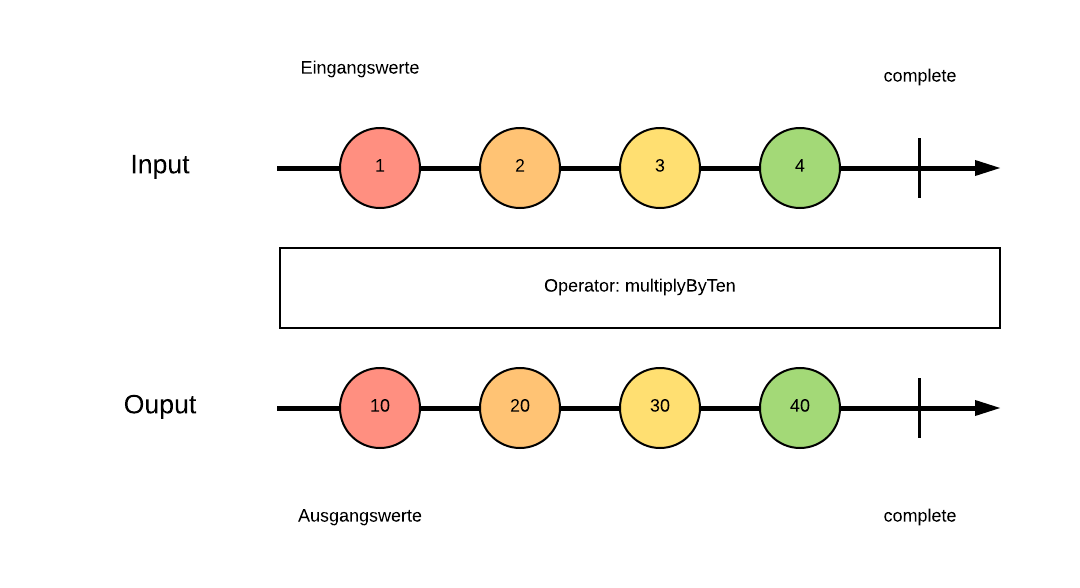
\includegraphics[width=12cm]{multiplybyten-fluss}
\end{figure}

\subsubsection{Instanz Operatoren und statische Operatoren}
Ein Instanz Operator, ist eine Methode die nur innerhalb einer Observable Instanz aufrufbar ist. Wenn die obige Methode eine offizielle Observable Methode sein würde, würde ihre Implementierung wie folgt aussehen:

\begin{figure}[H]
\begin{lstlisting}[basicstyle=\small]
RxJS.Observable.prototype.multiplyByTen = function() {
    const input = this;
    return RxJS.Observable.create(observer => input.subscribe(val => observer.next(val * 10),
        err => observer.error(err),
        () => observer.complete()
        )
    );
};
\end{lstlisting}
\caption{Implementation mit einem fiktiven Beispiel.}
\end{figure}

\noindent
Instanz Operatoren sind Funktionen die den \textbf{this} Ausdruck als Referenz des Input Observables nutzen. Das Input Observable wird nicht mehr als Callback genutzt, sondern als Funktionsaufruf eines Observable Objekts.

\begin{figure}[H]
\begin{lstlisting}[basicstyle=\small]
const source = RxJS.from([1, 2, 3, 4]).multiplyByTen();
source.subscribe(result => console.log(result));
\end{lstlisting}
\caption{Ausführung des selbsterstellten Observables.}
\end{figure}

\noindent
Ein statischer Operator hingegen ist eine Funktion, die direkt an die Observable-Klasse angehängt wird. Die typischsten statischen Operatoren sind die \textit{creation} Operatoren. Anstatt ein Input-Observable als Argument anzunehmen, wird ein nicht-Observable Objekt als Argument übergeben und somit ein neues Observable erstellt. Als Beispiel kann die Funktion interval genommen werden, die in Abbildung \ref{interval-obs} genutzt wurde. Sie nimmt einen numerischen Wert an und generiert ein neues Observable als Output. Weitere statische Kreationsoperatoren sind: \textbf{from()}, \textbf{range()}, \textbf{of()}, etc.

\subsubsection{Kategorien}

Es gibt Operatoren für verschiedene Anwendungsfälle und können kategorisiert werden in: Kreation, Transformierung, Multicasting, Kombination und Fehlerbehandlung. Wie ursprünglich bereits erwähnt werden Operatoren mit der pipe() Methode an einem Observable angeschlossen. Da die Kreations- und Multicasting-Operatoren bereits vorgestellt wurden, wird mit den Transformationsoperatoren fortgefahren.\\

\noindent
Um komplexe for Schleifen zu umgehen, bietet Javascript nativ die Möglichkeit mit Callback Funktionen Arrays weiterzuverarbeiten.

\begin{figure}[H]
\begin{lstlisting}[basicstyle=\small]
const source = ['1', '2', '5', 'foo', '13', '17', 'bar'];

console.log(source);

const result = source
    .map(val => parseInt(val, 10))
    .filter(num => !isNaN(num))
    .reduce((previous: number, current: number) => previous + current);
\end{lstlisting}
\caption{Die dargestellten Funktionen werden in der Praxis häufig verwendet um Arrays zu verarbeiten.}
\end{figure}

\noindent
In diesem Fall werden alle Werte in Zahlen umgewandelt und herausgefiltert. Letzteres wird die Summe gebildet. Observables bieten mit Operatoren die gleiche Funktionalität:

\begin{figure}[H]
\begin{lstlisting}[basicstyle=\small]
const result$ = from(source).pipe(
    map(val => parseInt(val, 10)),
    filter(num => !isNaN(num)),
    reduce((previous: number, current: number) => previous + current));

result$.subscribe(res => console.log(res));
\end{lstlisting}
\caption{Observable bieten Array-ähnliche Verarbeitungsmethoden.}
\end{figure}

\noindent
Mit dem Kreationsoperator from() wird jedes Iterable oder Promise Okjekt in einem Observable umgewandelt. Das Filtern der Zahlen und die anschließende Addition wurde unabhängig von externen Variablen und ganz mit Hilfe von puren Funktionen implementiert. Weitere Transformationsoperatoren sind unter Anderem \textbf{scan()}, \textbf{pluck()}, \textbf{switchMap()} etc.\\

\noindent
Ein häufiger Anwendungsfall ist asynchrone Operationen voneinander abhängig auszuführen. Wie in der Sektion Callbacks, Promises und Async await bereits gegenübergestellt, kann dieser Anwendungsfall auch mit Observables abgedeckt werden. Im folgenden werden die Kombinationsoperatoren vorgestellt die multiple Datenströme in verschiedensten Ausführungen verarbeiten oder kombinieren. Es werden die bisherigen Kapitelaufrufe als Beispiel genutzt. 

\begin{figure}[H]
\begin{lstlisting}[basicstyle=\small]
module.exports = {
    mode: 'development',
    entry: './src/modules/rxjs/stories-usage.ts',
    ...
}
\end{lstlisting}
\caption{Im Folgenden muss ../rxjs/stories-usage.ts als Eingangsdatei definiert werden.}
\end{figure}

\begin{figure}[H]
\begin{lstlisting}[basicstyle=\small]
export class HTTP {
    public makeRequest(url): Observable<any> {
        return from(new Promise((resolve, reject) => {
                const req = new XMLHttpRequest();
                req.open('GET', url);

                req.onload = () => {
                    if (req.status === 200) {
                        this.fakeLatency().then(() => resolve(JSON.parse(req.response)));
                    } else {
                        reject(Error(req.statusText));
                    }
                };

                req.onerror = () => {
                    reject(Error('Network Error'));
                };

                req.send();
            })
        );
    }
}

export class Story {
    ...
}

const story = new Story();
\end{lstlisting}
\caption{Das Praxisbeispiel der vorherigen Sektionen wird hier ebenfalls gegenübergestellt.}
\end{figure}

\noindent
Als einzige Änderung im Vergleich zum Beispiel der Sektion Promises, gibt in diesem Fall die makeRequest()-Methode kein Promise, sondern ein Observable zurück. Um die Kapitelaufrufe eins bis drei innerhalb einer Observable Sequenz auszugeben, würde der Code hierfür so aussehen:

\begin{figure}[H]
\begin{lstlisting}[basicstyle=\small]
from([1, 2, 3]).pipe(
    concatMap(chapter => story.getChapter(chapter)),
        tap(result => story.spawn(result)),
        finalize(() => story.displayFinished())
).subscribe();
\end{lstlisting}
\caption{Jeweils from() und concatMap() erstellen eigene Datenströme.}
\end{figure}

\noindent
Für jeden Wert den from() ausgibt, gibt concatMap() ein Observable zurück je nach angewendeter Funktion. In diesem Fall ist die angewendete Funktion story.getChapter(n). ConcatMap() flacht alle aus story.getChapter(n) resultierenden Observables zu einem zusammen. Somit werden alle entstandenen Ergebnisse der getChapter()-Aufrufe innerhalb einer Observable Sequenz zurückgegeben. Mit dem tap() Operator wird für jede Emission der Sequenz eine Nebenoperation ausgeführt. Tap() beeinflusst die Werte der Observable-Sequenz nicht. Schließlich wird vor Abschluss des Observables mit finalize() eine Funktion aufgerufen. Die Aktionen, die in tap() und finalize() durchgeführt werden, können auch durch den next() und dem complete() Callback des Observer Objekts ersetzt werden. In einem Marble-Diagramm abgebildet, wird deutlich, wie mit der Anwendung der Operatoren der Fluss verändert wird.

\begin{figure}[H]
\centering
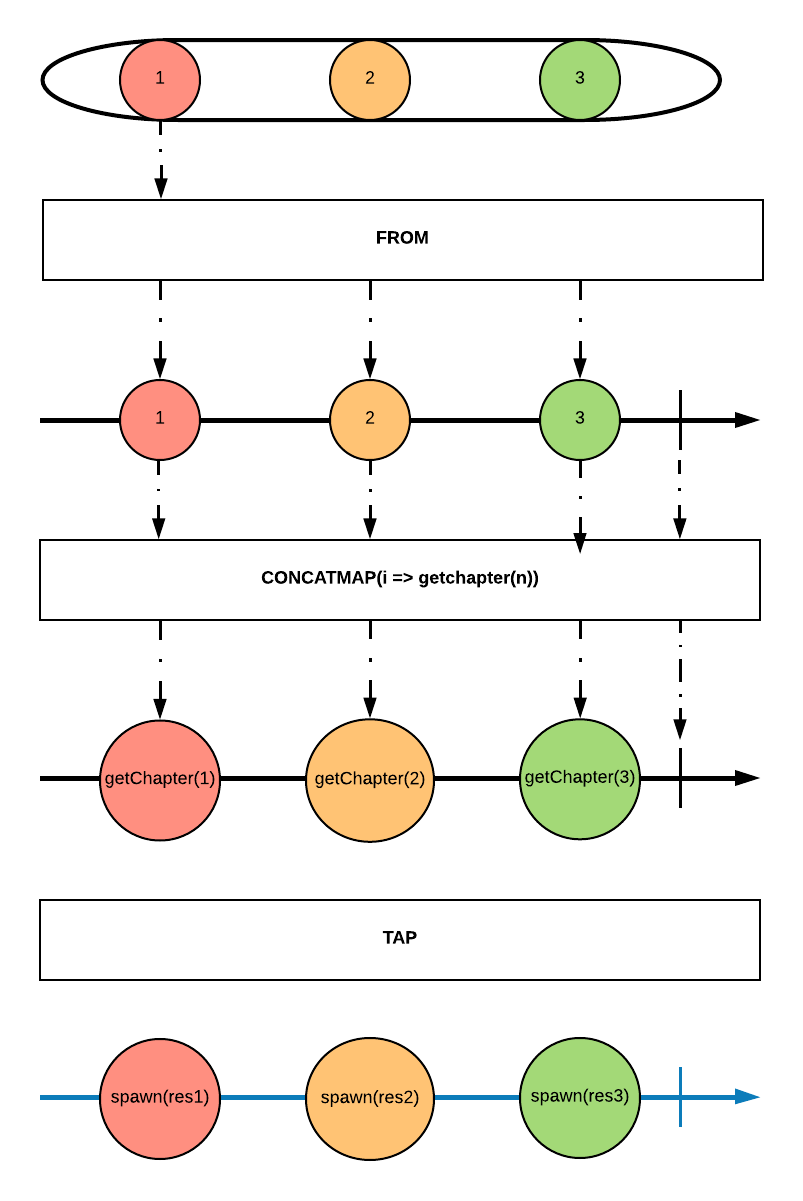
\includegraphics[width=8cm]{getchapters-fluss}
\caption{Finalize() ruft story.displayFinished() auf, wenn das Observable komplettiert.}
\end{figure}


\noindent
Es ist ebenfalls möglich Werte aus verschiedenen Observable Sequenzen gleichzeitig auszugeben. Mit dem statischen Operator \textbf{forkJoin()} kann ein Observable Array oder mehrere Observables als Argument übergeben werden. Sobald alle Observables erfolgreich ihre Werte emittiert haben und die Sequenzen abgeschlossen sind, werden die gesamte Anzahl an Werten an die Observer verteilt. Forkjoin() führt die Observables in der Reihenfolge aus, in der sie als Argument übergeben worden sind. Dementsprechend wird auf jede Sequenz gewartet bis die Werte ausgegeben und das Observable fertiggestellt wird. Somit addiert sich die Zeit bis alle Sequenzen abgeschlossen sind. Observables forkJoin() ist das Gegenstück zum \textbf{Promise.all()}. Es gibt noch zahlreiche weitere Operatoren die mehrere Observables kombinieren können. Dazu gehören unter anderem \textbf{MergeMap()}, \textbf{concat()}, \textbf{merge()}, \textbf{combineLatest()} etc.\\


\noindent
Als letzte aber nicht unwesentlich wichtige Kategorie wird die Fehlerbehandlung mit Observables abgedeckt. Bei selbsterstellten Observables werden Fehler mit der error() Funktion an die Observer übergeben (siehe Abb. \ref{catch-error-obs}). Observer verarbeiten daraufhin innerhalb der subscribe() Methode mit dem error() Callback jeden ankommenden Fehler. Mit Operatoren ist es möglich Fehler zwischen der Verarbeitung zu werfen oder zu fangen:

\begin{figure}[H]
\begin{lstlisting}[basicstyle=\small]
from([1, 2, 3]).pipe(
    concatMap(chapter => {
        if (chapter === 3) {
            return throwError(new Error('Forced error!'));
        } else {
            return story.getChapter(chapter);
        }
    }),
    catchError((err) => {
        console.error(err);
        return of([{title: 'Fallback title', id: 101, body: 'Fallback body'}]);
    })
).subscribe({
    next: val => story.spawn(val),
    complete: () => story.displayFinished()
});
\end{lstlisting}
\caption{CatchError() ist in diesem Fall keine selbsterstellte Methode der Klasse Story, sondern ein Observable Operator.}
\end{figure}

\noindent
In diesem Beispiel wird der Auftritt eines Fehlers mit throwError() simuliert und mit catchError() gefangen. Ein in der Praxis öfters verwendeter Operator ist \textbf{retry()}. Da nach einer Emission eines Fehler eine Subscription abläuft, wird mit retry(count) die Subscription wieder neu initiiert. Die Anzahl an Neuversuche einer Subscription wird vom übergebenen Parameter bestimmt.\\

\noindent
Wie man nun gesehen hat bilden Operatoren etliche Möglichkeiten das Verhalten von Observables zu beeinflussen. Die angeführten Beispiele waren nur die Spitze des Eisbergs. Alle Operatoren abzudecken, würde jedoch den Rahmen sprengen. Um mehr von Operatoren zu erfahren, kann in der Dokumentation von RxJS nachgeschaut werden:

\begin{center}
\url{http://reactivex.io/rxjs/manual/overview.html#operators} 
\end{center}

\subsection{Optional: Wikipedia Such-App}


\subsection{Fazit}
RxJS und das Prinzip der reaktiven Programmierung zu lernen kann hart sein. Speziell RxJS bietet eine riesige API und verlangt ein umdenken vom imperativen- zum deklarativen Programmierstil. Ohne einem fundamentalen Wissensstand wie Observables intern funktionieren, kann durchaus gedacht werden, dass RxJS viel \glqq Magie\grqq{} praktiziert. Diese Sektion sollte eine Einführung in die Konzeption eines Observables geben. Als Faustregel: Observables können sowohl synchron als auch asynchron agieren. Im Gegensatz zu Funktionen können mehrere Werte mit der Zeit ausgegeben werden. Sinnbildlich kann man ein Observable mit einem Array gleichsetzen, dass mit der Zeit Werte erstellt. Funktionen, die mit dieser speziellen Form eines Array operieren, haben die Möglichkeit auf neu entstandene Werte zuzugreifen. Unterschiedliche Observable Typen offenbaren unterschiedliche Verhaltensmechanismen. Observables können cold oder hot sein. Cold Observables rufen den Datenproduzenten beim Start einer Subscription auf. Infolgedessen bekommt jeder Observer einen eigene Sequenz an Werten vom Datenproduzenten zugesprochen. Bei einer Subscription eines hot Observables hingegen, kann es durchaus sein, dass obwohl Werte erwartet werden, keine ankommen. In diesem Fall bekommen alle Observer die gleiche Sequenz an Werten und wenn spät angeschlossene Observer sich anschließen - können diese mögliche Werte verpassen. Eine spezielle Form von Observables sind Subjects. Subjects sind von vornherein multicasting fähig. Das bedeutet, angeschlossene Observer werden in einer Liste von Observer registriert und alle registrierten Observer bekommen die gleiche Exekution des Datenproduzenten. Zudem können Subjects als Observable oder als Observer operieren. Deshalb ist es auch Möglich ein Subject Objekt als Argument einer subscribe() Methode zu übergeben. Schedulers finden in RxJS selten an Anwendung. Mit Ihnen kann man steuern wann ein Observable seine Observer benachrichtigt. Um dies zu ermöglichen arbeiten Schedulers mit einer virtuellen Uhr.

